\subsection{Introduzione}
Questa sezione ha lo scopo di descrivere i vari casi d'suo che sono stati identificati dal gruppo Bug's Bunny 
come delle potenziali funzionalità dell'applicazione.

\subsection{Attori}
\begin{itemize}
    \item \textbf{Utente non registrato}: 
    è un utente che non ha ancora effettuato la registrazione presso l'applicativo. 
    Non possiede credenziali per effettuare l'autenticazione presso la piattaforma e non ha accesso a nessuna funzionalità dell'applicazione  
    \item \textbf{Utente non autenticato}
    è un utente che ancora deve autenticarsi nell'applicazione. Può essere in possesso di credenziali di accesso oppure no.
    \item \textbf{Utente autenticato}
    è un utente che ha effettuato l'autenticazione della piattaforma ed ha accesso alle funzionalità di essa.
\end{itemize}

\begin{figure}[!h]
    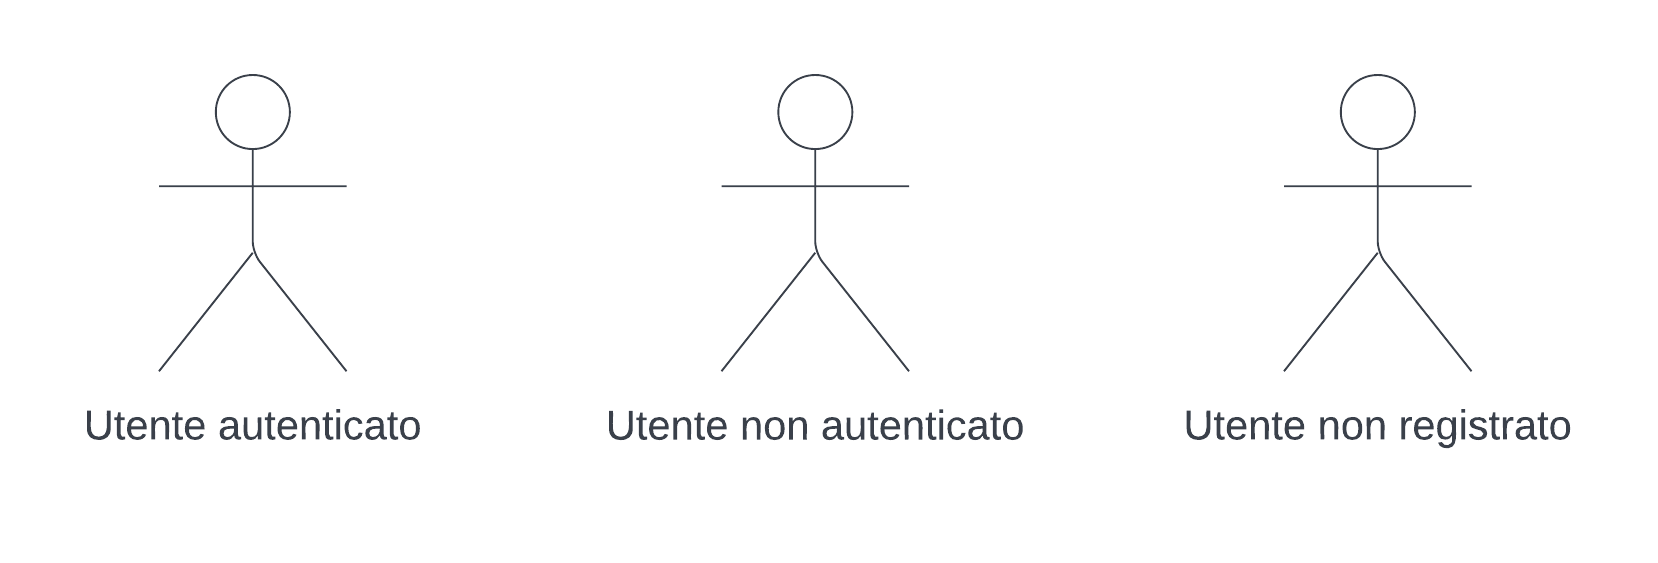
\includegraphics[width=10cm]{sezioni/Images/Actors.png}
    \centering
    \caption{Gerarchia attori}
\end{figure}
\newpage
    
\subsection{UC 1 - Registrazione manuale}

\begin{figure}[!h]
    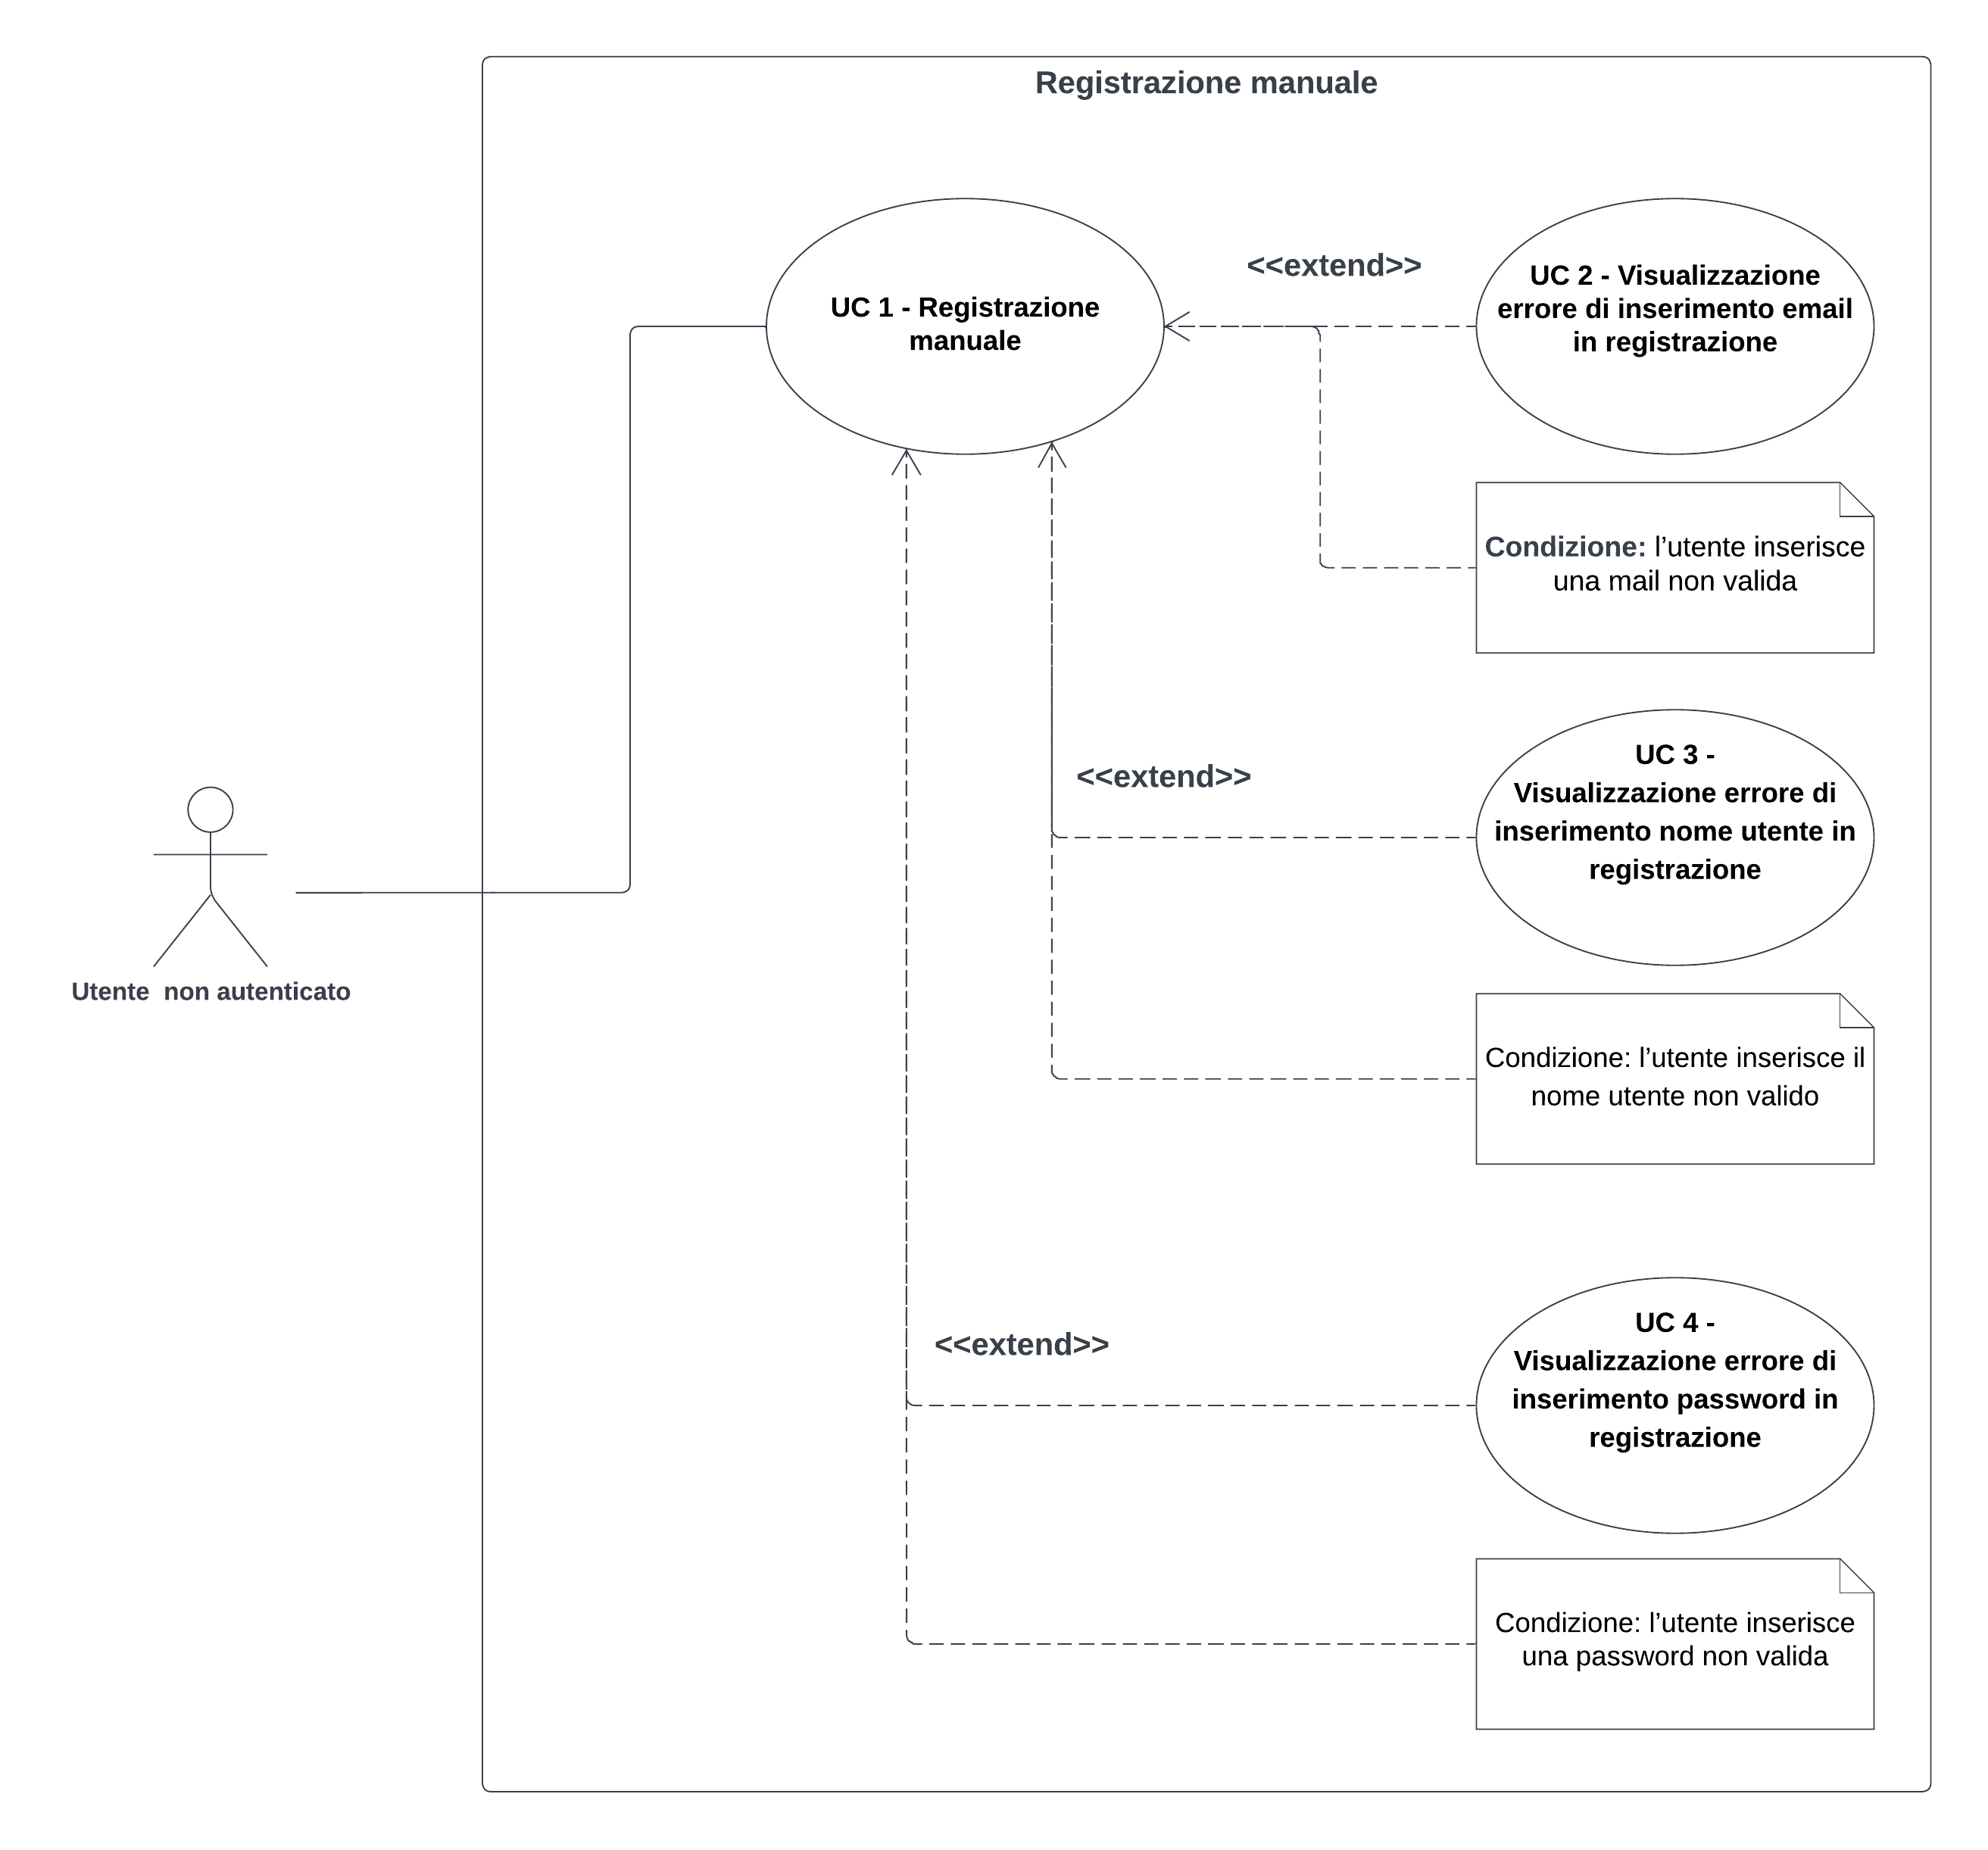
\includegraphics[width=15cm]{sezioni/Images/UC1.png}
    \centering
    \caption{UC 1 - Registrazione manuale}
\end{figure}

\begin{itemize}
    \item \textbf{Attore}: utente non registrato.
    \item \textbf{Descrizione}: l’utente deve poter avere la possibilità di creare un account personale.
    \item \textbf{Scenario}:
    \begin{enumerate}
        \item l’utente si collega al sistema;
        \item l’utente clicca sul pulsante di registrazione;
        \item l’utente inserisce la propria email \textbf{(UC 1.1)};
        \item l’utente inserisce il proprio nome utente \textbf{(UC 1.2)};
        \item l’utente inserisce una password \textbf{(UC 1.3)};
        \item l’utente conferma i dati inseriti per proseguire.
    \end{enumerate}
    \item \textbf{Estensioni}:
        - l’utente inserisce una mail non valida  \textbf{(UC 2)};\\
        - l’utente inserisce il nome utente non valido \textbf{(UC 3)};\\
        - l’utente inserisce una password non valida \textbf{(UC 4)};\\

    \item \textbf{Precondizioni}: l’utente non è ancora registrato nel sistema.
    \item \textbf{Postcondizioni}: l’utente è registrato nel sistema.
\end{itemize}

\subsubsection{UC 1.1 - Inserimento email}
\begin{itemize}
    \item \textbf{Attore}: utente non registrato.
    \item \textbf{Descrizione}: l’utente deve avere la possibilità di inserire l’email.
    \item \textbf{Scenario}:
    \begin{enumerate}
        \item l’utente seleziona il campo relativo alla mail;
        \item l’utente inserisce la propria email.
    \end{enumerate}

    \item \textbf{Precondizioni}: l’utente effettua l’attività di registrazione.
    \item \textbf{Postcondizioni}: l’utente ha compilato il campo relativo alla mail.
\end{itemize}

\subsubsection{UC 1.2 - Inserimento nuovo nome utente}
\begin{itemize}
    \item \textbf{Attore}: utente non registrato.
    \item \textbf{Descrizione}: l’utente deve avere la possibilità di creare un nuovo nome utente.
    \item \textbf{Scenario}:
    \begin{enumerate}
        \item l’utente seleziona il campo relativo il nuovo nome utente;
        \item l’utente crea il proprio nuovo nome utente.
    \end{enumerate}

    \item \textbf{Precondizioni}: l’utente effettua l’attività di registrazione.
    \item \textbf{Postcondizioni}: l’utente ha compilato il campo relativo il nuovo nome utente.
\end{itemize}

\subsubsection{UC 1.3 - Inserimento nuova password}
begin{itemize}
    \item \textbf{Attore}: utente non registrato.
    \item \textbf{Descrizione}: l’utente deve avere la possibilità di creare una nuova password.
    \item \textbf{Scenario}:
    \begin{enumerate}
        \item l’utente seleziona il campo relativo la nuova password;
        \item l’utente crea la nuova password.
    \end{enumerate}

    \item \textbf{Precondizioni}: l’utente effettua l’attività di registrazione.
    \item \textbf{Postcondizioni}: l’utente ha compilato il campo relativo la nuova password.
\end{itemize}


\begin{figure}[!h]
    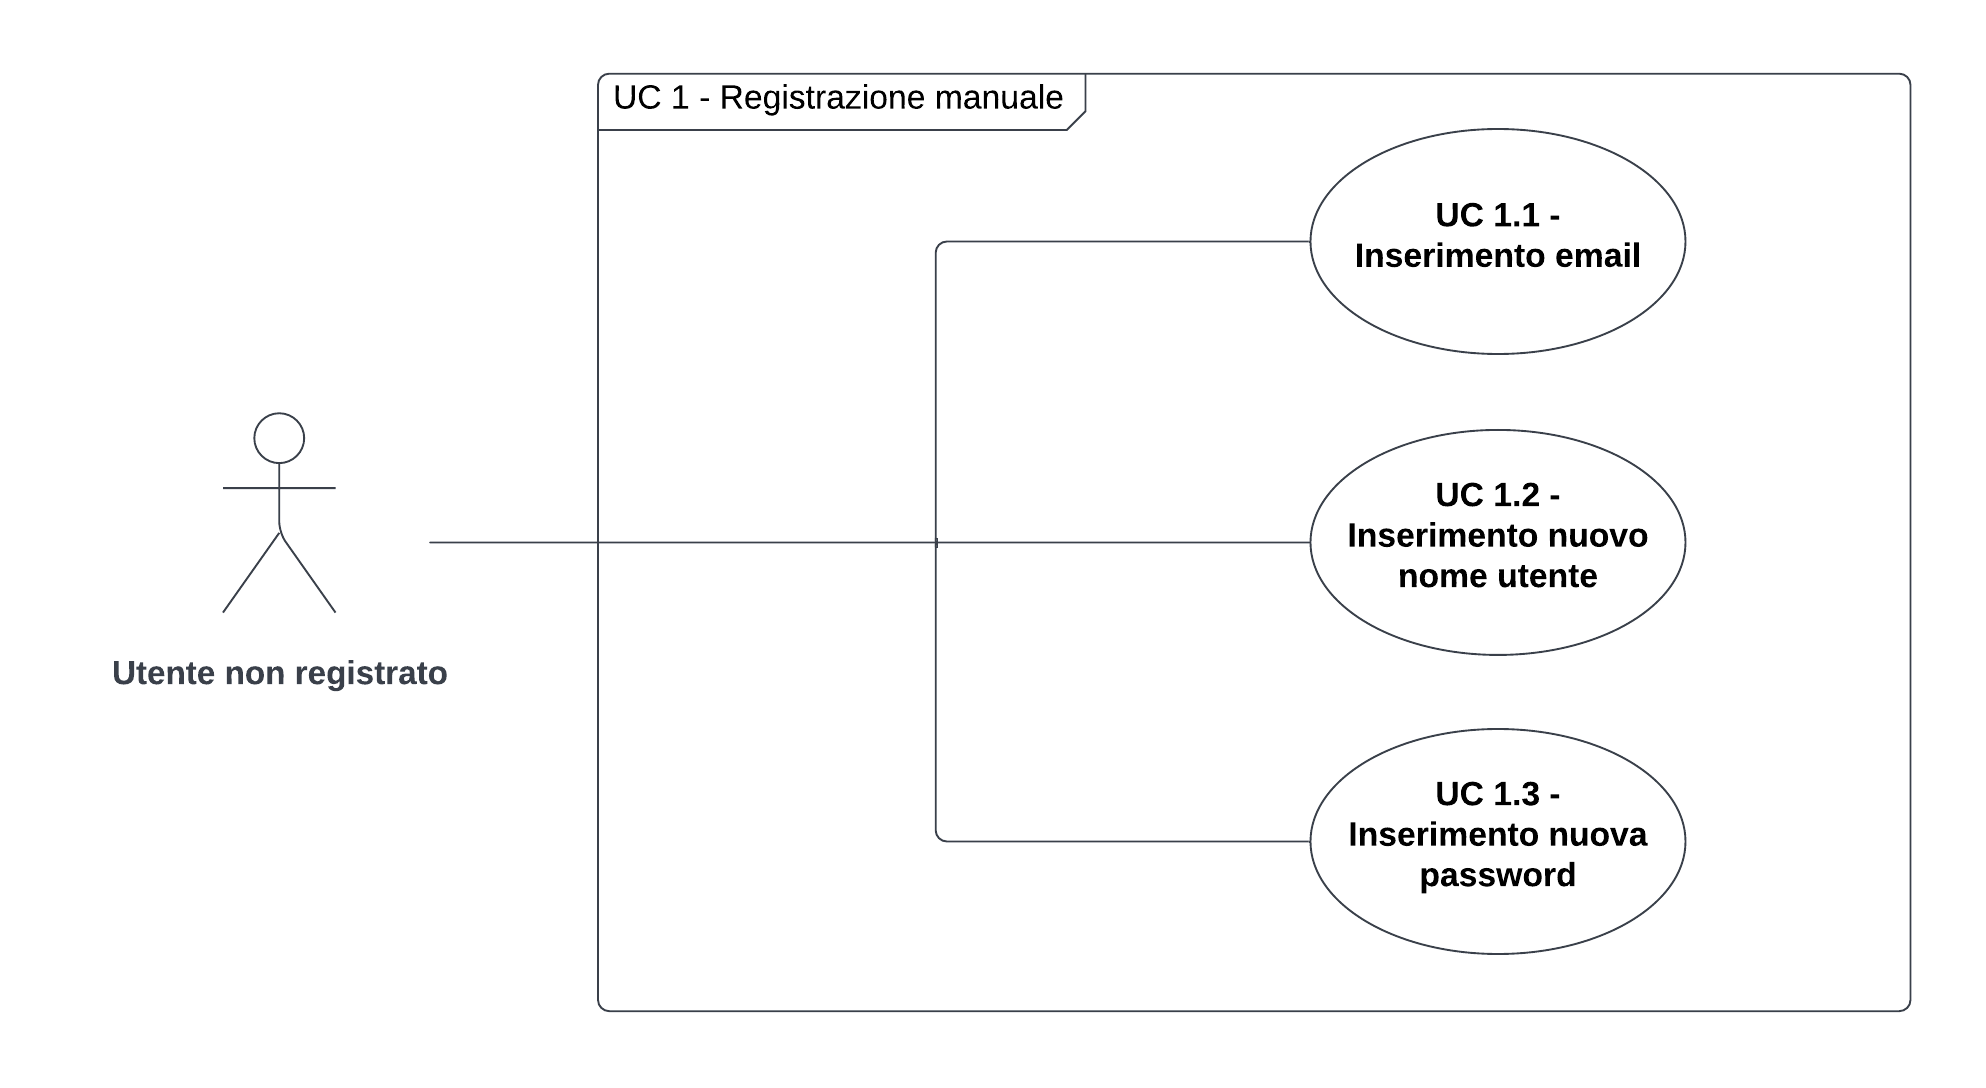
\includegraphics[width=15cm]{sezioni/Images/UC1_s.png}
    \centering
    \caption{Registrazione manuale}
\end{figure}

\subsection{UC 2 - Visualizzazione errore di inserimento email in registrazione}
begin{itemize}
    \item \textbf{Attore}: utente non registrato.
    \item \textbf{Descrizione}: l’utente deve essere notificato con un errore nel caso in cui le informazioni inserite nel campo email siano invalide.
    \item \textbf{Scenario}: L’utente visualizza un messaggio di errore.
    \item \textbf{Precondizioni}: l’utente inserisce una mail non valida nell'apposito input box.
    \item \textbf{Postcondizioni}: l’utente riceve il messaggio di errore.
\end{itemize}

\subsection{UC 3 - Visualizzazione errore di inserimento nome utente in registrazione}
begin{itemize}
    \item \textbf{Attore}: utente non registrato.
    \item \textbf{Descrizione}: l’utente deve essere notificato con un errore nel caso in cui venga inserito un nome utente non valido.
    \item \textbf{Scenario}: L’utente visualizza un messaggio di errore.
    \item \textbf{Precondizioni}: l’utente inserisce un nome utente non valido nell'apposito input box.
    \item \textbf{Postcondizioni}: l’utente riceve il messaggio di errore.
\end{itemize}

\subsection{UC 4 - Visualizzazione errore di inserimento password in registrazione}
begin{itemize}
    \item \textbf{Attore}: utente non registrato.
    \item \textbf{Descrizione}: l’utente deve essere notificato con un errore nel caso in cui inserisca una password non valida durante la fase di registrazione.
    \item \textbf{Scenario}: L’utente visualizza un messaggio di errore.
    \item \textbf{Precondizioni}: l’utente inserisce una password non valida nell'apposito input box.
    \item \textbf{Postcondizioni}: l’utente riceve il messaggio di errore.
\end{itemize}

\subsection{UC 5 - Login manuale}
\begin{figure}[!h]
    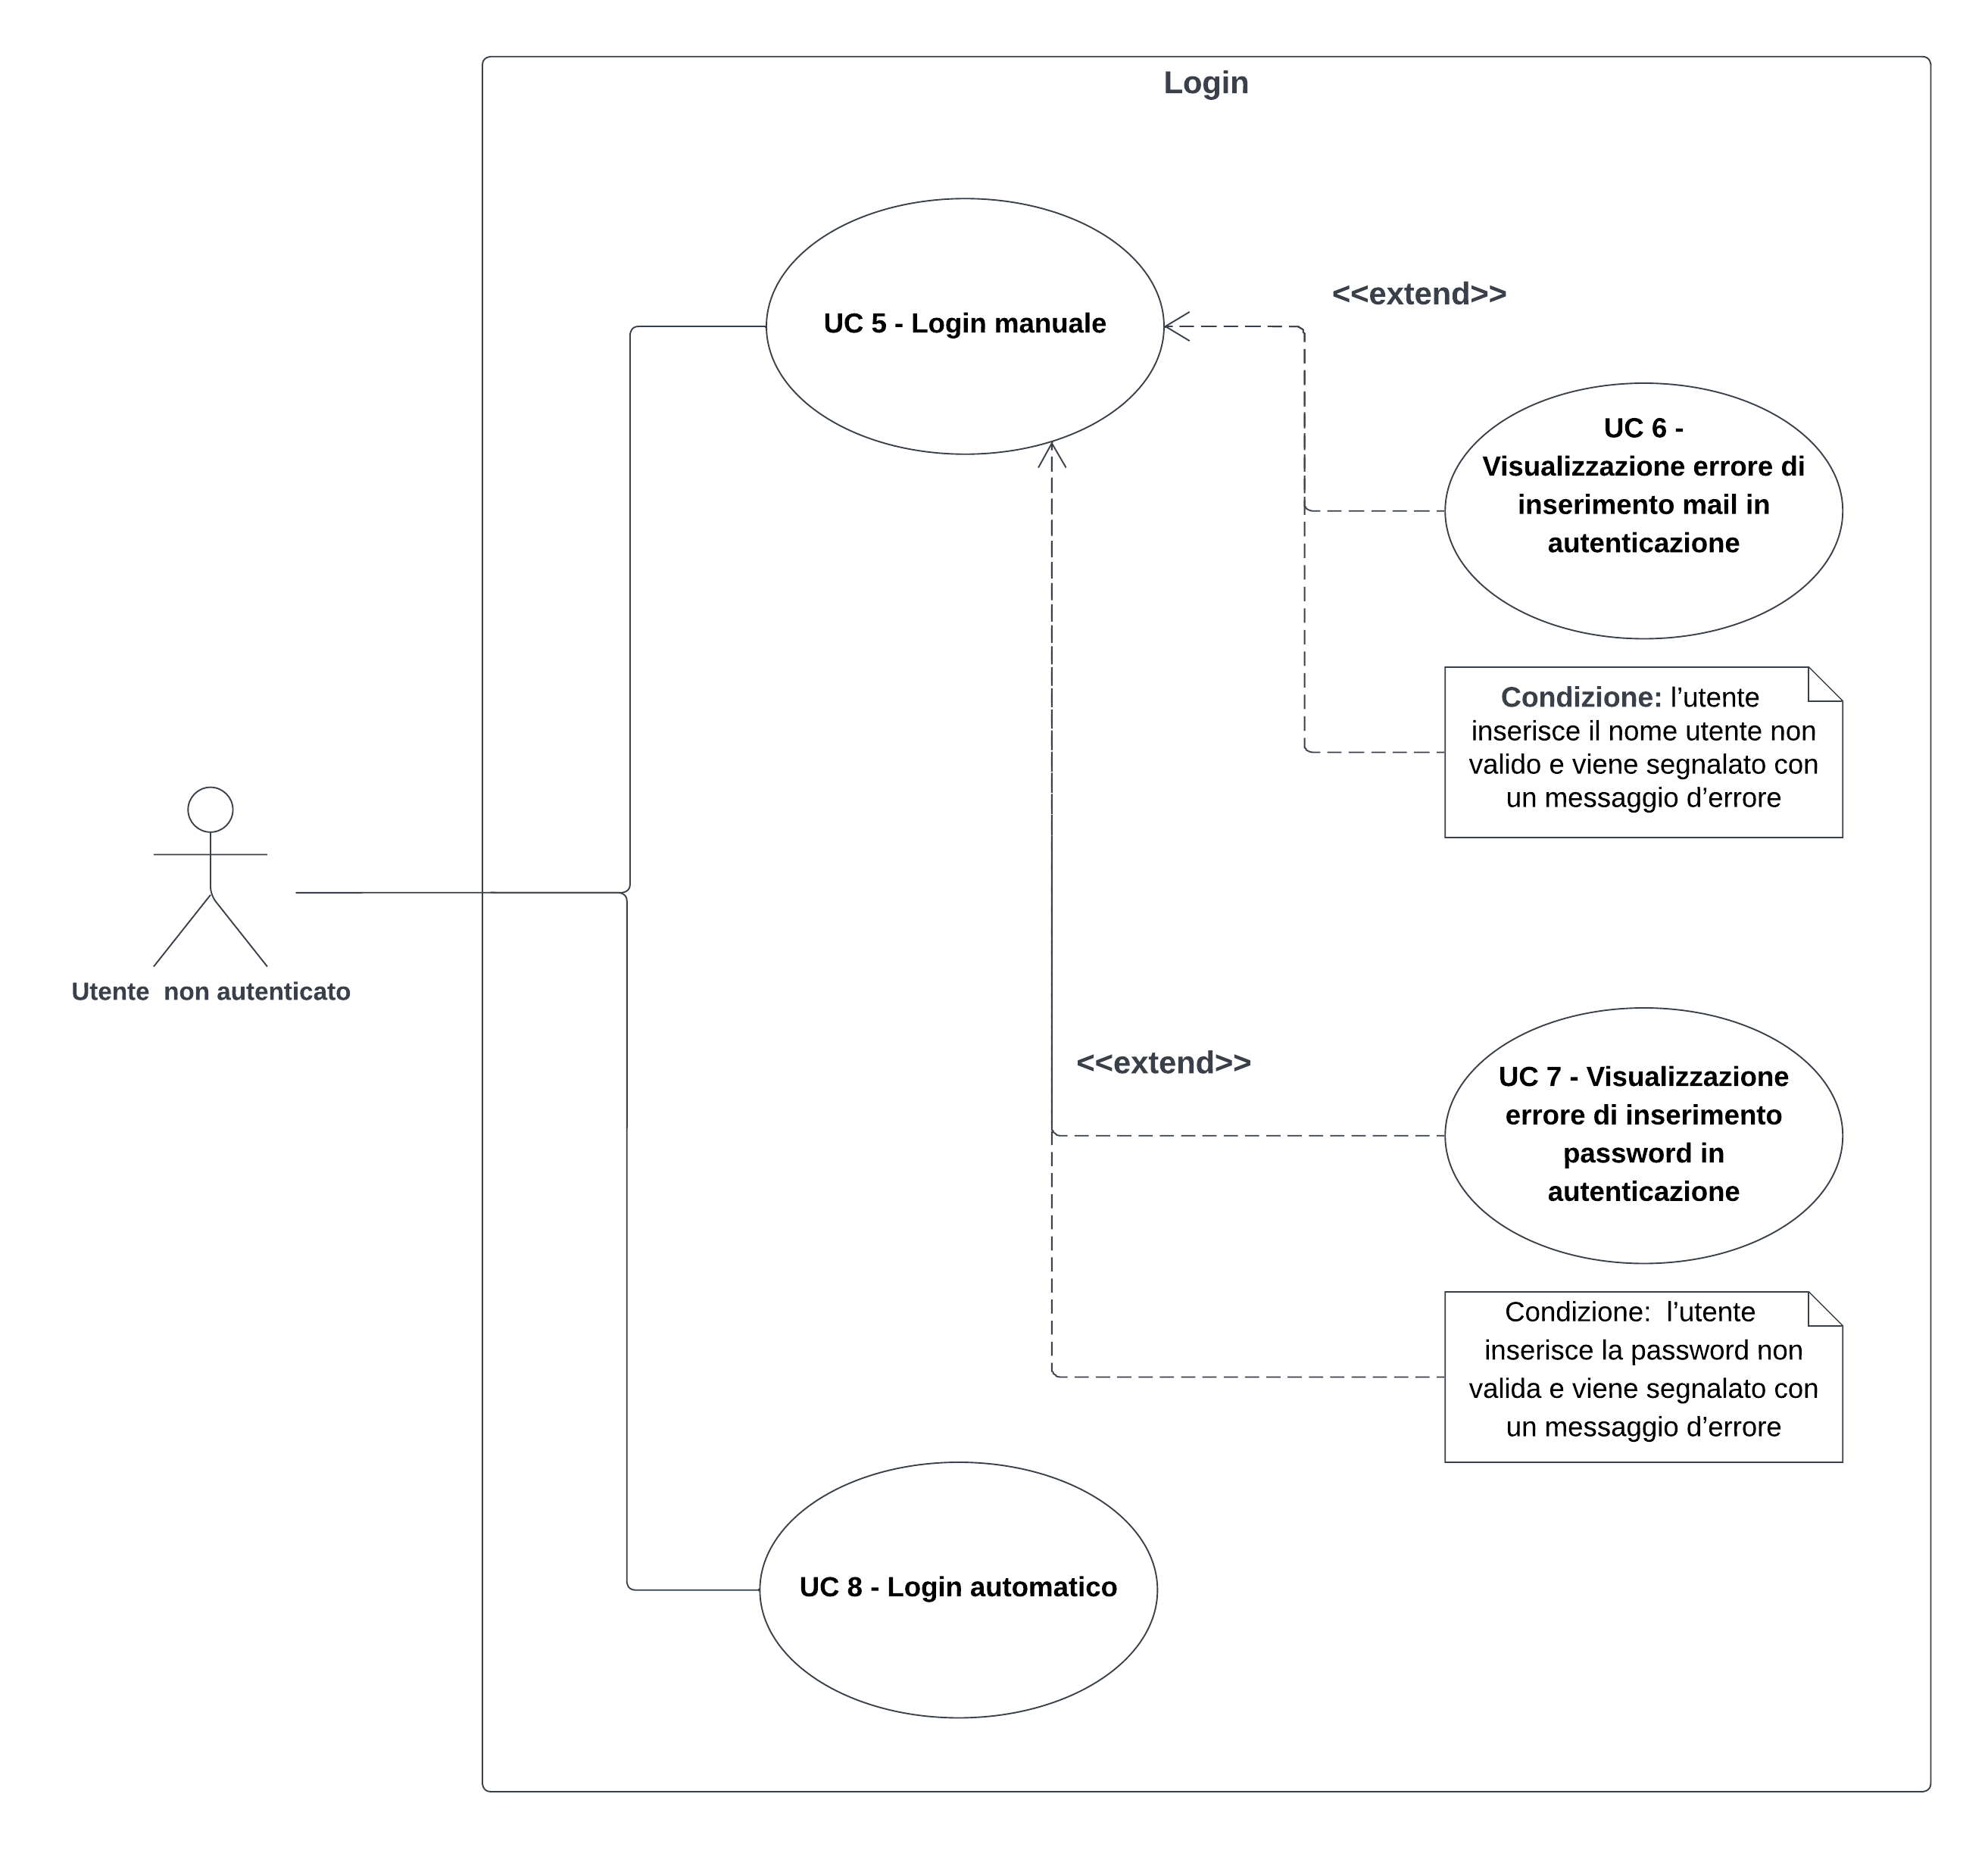
\includegraphics[width=10cm]{sezioni/Images/UC5.png}
    \centering
    \caption{UC 5 - Login manuale}
\end{figure}

\begin{itemize}
    \item \textbf{Attore}: l’utente non è autenticato.
    \item \textbf{Descrizione}: l’utente accedendo con l’account personale, deve poter autenticarsi.
    \item \textbf{Scenario}:
    \begin{enumerate}
        \item l’utente si collega al sistema;
        \item l’utente clicca sul pulsante di login;
        \item l’utente inserisce il proprio nome utente \textbf{(UC 5.1)};
        \item l’utente inserisce la propria password \textbf{(UC 5.2)};
        \item l’utente decide se memorizzare la sessione \textbf{(UC 5.3 )};
        \item l’utente clicca il pulsante di conferma per proseguire.
    \end{enumerate}
    \item \textbf{Estensioni}:
        - l’utente inserisce il nome utente non valido e viene segnalato con un messaggio d’errore \textbf{(UC 6)};\\
        - l’utente inserisce la password non valida e viene segnalato con un messaggio d’errore \textbf{(UC 7)};\\

    \item \textbf{Precondizioni}: l’utente non è ancora autenticato.
    \item \textbf{Postcondizioni}: l’utente si è autenticato al sistema.
\end{itemize}

\subsubsection{UC 5.1 - Inserimento nome utente}
begin{itemize}
    \item \textbf{Attore}: utente non autenticato.
    \item \textbf{Descrizione}: l’utente deve poter inserire il nome utente per autenticarsi.
    \item \textbf{Scenario}:
    \begin{enumerate}
        \item l’utente seleziona il campo relativo al nome utente;
        \item l’utente inserisce il nome utente.
    \end{enumerate}

    \item \textbf{Precondizioni}: l’utente effettua l’attività di autenticazione.
    \item \textbf{Postcondizioni}: l’utente ha compilato il campo relativo il nome utente.
\end{itemize}

\subsubsection{UC 5.2 - Inserimento password}
Attore: utente non autenticato
Descrizione: l’utente deve poter inserire la password per autenticarsi
Scenario: 
l’utente seleziona il campo relativo alla password
l’utente inserisce la password
Precondizioni: l’utente effettua l’attività di autenticazione
Postcondizioni: l’utente ha compilato il campo relativo la password
Estensioni (eventuali): la password inserita deve essere corretta altrimenti comparirà un messaggio d’errore. 

\subsubsection{UC 5.3 Memorizzazione sessione}
Attore: utente non autenticato
Descrizione: l’utente deve poter memorizzare la sessione.
Scenario: l’utente spunta la casella per mantenere memorizzata la sessione.
Precondizioni: l’utente effettua l’attività di autenticazione.
Postcondizioni: l’utente ha chiesto che la sessione venga memorizzata.


\subsection{UC 6 - Visualizzazione errore di inserimento mail in autenticazione}
Attore: utente non autenticato
Descrizione: l’utente deve essere notificato con un errore nel caso in cui l’email inserita sia invalida durante la fase di autenticazione.
Scenario: L’utente visualizza un messaggio di errore. 
Precondizioni: l’utente effettua l’attività di autenticazione ed inserisce l’email non valida.
Postcondizioni: l’utente riceve il messaggio di errore.

\subsection{UC 7 - Visualizzazione errore di inserimento password in autenticazione} 
Attore: utente non autenticato
Descrizione: l’utente deve essere notificato con un errore nel caso in cui la password inserita sia invalida durante la fase di autenticazione.
Scenario: L’utente visualizza un messaggio di errore. 
Precondizioni: l’utente effettua l’attività di autenticazione ed inserisce la password non valida.
Postcondizioni: l’utente riceve il messaggio di errore.

\subsection{UC 8 - Login automatico}
Attore: l’utente non è autenticato 
Descrizione: l’utente accedendo con l’account personale, deve poter autenticarsi automaticamente se la sessione rimane memorizzata
Scenario:
l’utente si collega al sistema 
l’utente viene automaticamente autenticato 
Precondizioni: l’utente ha una sessione attiva memorizzata
Postcondizioni: l’utente si è autenticato al sistema

\subsection{UC 9 - Logout}
Attore: l’utente è autenticato 
Descrizione: l’utente deve poter uscire dalla sessione
Scenario:
l’utente è collegato al sistema
l’utente clicca il pulsante di logout
Estensioni: /
Precondizioni: l’utente è autenticato
Postcondizioni: l’utente non è più autenticato al sistema

\subsection{UC 10 - Modifica password}
Attore: l’utente è autenticato
Descrizione: l’utente deve poter modificare l’attuale password, con la quale effettua il login
Scenario:
Inserimento psw attuale
Inserimento nuova psw
Conferma nuova psw
Conferma modifica psw
Estensioni: 
l’utente inserisce l’attuale password e non coincide con quella attuale, viene visualizzato un messaggio di errore (UC 11)
l’utente inserisce la nuova password ma essa non rispetta determinate condizioni quindi viene visualizzato un messaggio di errore (UC 12)
l’utente non inserisce in modo corretto la nuova password nella conferma della stessa, quindi viene visualizzato un messaggio di errore (UC 13)
Precondizioni: l’utente è autenticato con una determinata password
Postcondizioni l’utente è autenticato con una nuova password

\subsubsection{UC 10.1 - Inserimento password attuale} 
Attore: utente autenticato
Descrizione: l’utente deve inserire la password attuale durante la sessione di “modifica password”
Scenario
l’utente seleziona il campo riferito alla password attuale
l’utente inserisce la password attuale
Precondizioni: l’utente svolge la sessione di modifica password
Postcondizioni: l’utente ha inserito la propria password attuale

\subsubsection{UC 10.2 - Inserimento nuova password}
Attore: utente autenticato
Descrizione: durante l’attività di modifica password l’utente deve poter inserire la nuova password
Scenario: 
l’utente seleziona il campo riferito alla nuova password
l’utente inserisce la nuova password 
Precondizioni:l’utente svolge la sessione di modifica password
Postcondizioni:l’utente ha inserito la nuova password 

\subsubsection{UC 10.3 Inserimento ripetizione nuova password}
Attore: utente autenticato
Descrizione: durante l’attività di modifica password l’utente deve poter inserire la ripetizione della nuova password
Scenario: 
l’utente seleziona il campo riferito alla ripetizione della nuova password
l’utente inserisce la ripetizione della nuova password 
Precondizioni:l’utente svolge la sessione di modifica password
Postcondizioni:l’utente ha inserito la ripetizione della nuova password 

\subsubsection{UC 10.4 - Conferma modifica password}
Attore: utente autenticato
Descrizione: durante l’attività di modifica password l’utente deve poter confermare la nuova password
Scenario: l’utente conferma la nuova password inserita
Precondizioni:l’utente svolge la sessione di modifica password
Postcondizioni:l’utente ha provato a modificare la propria password

\subsection{UC 11 - Visualizzazione errore di inserimento password attuale}
Attore: utente autenticato
Descrizione: durante l’attività di modifica password l’utente deve ricevere un messaggio d’errore se l'inserimento della password attuale non è andato a buon fine
Scenario: l’utente legge un messaggio d’errore
Precondizioni:l’utente svolge la sessione di modifica password e la password attuale inserita non è corretta
Postcondizioni:l’utente ha ricevuto un messaggio d’errore

\subsection{UC 12 - Visualizzazione errore di inserimento nuova password non valida}
Attore: utente autenticato
Descrizione: durante l’attività di modifica password l’utente deve ricevere un messaggio d’errore se l'inserimento di una nuova password non è valida
Scenario: l’utente legge un messaggio d’errore
Precondizioni:l’utente svolge la sessione di modifica password e la nuova password inserita non è valida
Postcondizioni:l’utente ha ricevuto un messaggio d’errore

\subsection{UC 13 - Visualizzazione errore di ripetizione nuova password}
Attore: utente autenticato
Descrizione: durante l’attività di modifica password l’utente deve ricevere un messaggio d’errore se l'inserimento della ripetizione della nuova password non è uguale alla nuova password 
Scenario: l’utente legge un messaggio d’errore
Precondizioni:l’utente svolge la sessione di modifica password e la ripetizione della nuova password inserita non è corretta
Postcondizioni:l’utente ha ricevuto un messaggio d’errore

\subsection{UC 14 - Visualizzazione guida}
Attore: utente autenticato
Descrizione: l’utente deve poter visualizzare la guida in formato mappa o formato lista
Scenario:
l’utente si trova nella home
Precondizione: l’utente vuole visualizzare la guida
Postcondizione: l’utente visualizza la guida

\subsubsection{UC 14.1 - Visualizzazione mappa globale}
Attore: utente autenticato
Descrizione: l’utente visualizza la mappa globale se non ha nessun profilo social seguito
Scenario:
l’utente non segue nessun profilo social
l’utente visualizza la mappa globale nella home

\subsubsection{UC 14.2 - Visualizzazione lista globale}
Attore: utente autenticato
Descrizione: l’utente visualizza la lista globale se non ha nessun profilo social seguito
Scenario:
l’utente non segue nessun profilo social
l’utente visualizza la lista globale nella home

\subsubsection{UC 14.3 - Visualizzazione mappa personalizzata}
Attore: utente autenticato
Descrizione: l’utente visualizza la mappa personalizzata se ha dei profili social seguiti
Scenario:
l’utente segue dei profilo social
l’utente visualizza la mappa personalizzata nella home

\subsubsection{UC 14.4 - Visualizzazione lista personalizzata}
Attore: utente autenticato
Descrizione: l’utente visualizza la lista personalizzata se ha dei profili social seguiti
Scenario:
l’utente segue dei profilo social
l’utente visualizza la lista personalizzata nella home

\subsection{UC 15 - Inserimento profili social da seguire}
Attore: utente autenticato
Descrizione: l’utente deve poter aggiungere dei profili social da seguire e da cui sarà generata la guida
Scenario:
l’utente naviga nella sezione dei profili seguiti
l’utente clicca il pulsante di aggiunta profile
l’utente sceglie instagram o tiktok
l’utente inserisce l’username
l’utente conferma e salva
Estensioni:
il profilo inserito non esiste (UC 16)
il profilo inserito è già stato aggiunto (UC 17)
Precondizione: l’utente vuole seguire un nuovo utente
Postcondizione: l’utente ha inserito un nuovo utente da seguire


\subsection{UC 16 - Visualizzazione errore di nome utente non esistente}
Attore: utente autenticato
Descrizione: durante l’attività di aggiunta di un profilo l’utente deve ricevere un messaggio d’errore se il nome utente ricercato non è presente nel sistema
Scenario: l’utente legge un messaggio d’errore
Precondizioni:l’utente inserisce un nome utente inesistente nella procedura di inserimento dei profli social da seguire
Postcondizioni:l’utente ha ricevuto un messaggio d’errore

\subsection{UC 17 - Visualizzazione errore di utente già presente nel sistema}
Attore: utente autenticato
Descrizione: durante l’attività di aggiunta di un profilo l’utente deve ricevere un messaggio d’errore se il nome utente ricercato è già stato inserito nei profili seguiti dall’utente
Scenario: l’utente legge un messaggio d’errore
Precondizioni:l’utente inserisce un nome utente nella procedura di inserimento dei profli social da seguire che è già presente tra quelli seguiti.
Postcondizioni:l’utente ha ricevuto un messaggio d’errore

\subsection{UC 18 - Rimozione profili social seguito}
Attore: utente autenticato
Descrizione: l’utente deve poter rimuovere un profilo dalla lista di quelli seguiti
Scenario:
l’utente naviga nella sezione dei profili seguiti
l’utente seleziona il profilo che vuole rimuovere
l’utente clicca il pulsante di rimozione
Precondizione: l’utente vuole rimuovere un profilo social dalla lista dei seguiti
Postcondizione: l’utente ha rimosso il profilo social dalla lista dei seguiti

\subsection{UC 19 - Esplorazione profili social più seguiti}
Attore: utente autenticato
Descrizione: l’utente può esplorare gli utenti più seguiti dagli altri utenti di questa piattaforma
Scenario: 
l’utente si trova nella home
l’utente preme il pulsante per entrare nella pagina di esplorazione
l’utente vede la lista degli utenti più seguiti sia di instagram che di tiktok
Precondizione: l’utente vuole visualizzare gli utenti più seguiti
Postcondizione: viene visualizzata all’utente la lista degli utenti più seguiti

\subsection{UC 20 - Impostazione vista predefinita guida}
Attore: utente autenticato
Descrizione: l’utente deve poter scegliere la vista predefinita per visualizzare la guida
Scenario: 
l’utente naviga nella sezione impostazioni
l’utente sceglie la voce “Vista predefinita”

\subsubsection{UC 20.1 - Impostazione mappa come vista predefinita}
Attore: utente autenticato
Descrizione: l’utente sceglie la mappa come vista predefinita
Scenario:
l’utente sceglie mappa come vista predefinita
Precondizione: l’utente vuole scegliere mappa come vista predefinita
Postcondizione: mappa viene impostata come vista predefinita

\subsubsection{UC 20.2 - Impostazione lista come vista predefinita}
Attore: utente autenticato
Descrizione: l’utente sceglie la lista come vista predefinita
Scenario:
l’utente sceglie lista come vista predefinita
Precondizione: l’utente vuole scegliere lista come vista predefinita
Postcondizione: lista viene impostata come vista predefinita





